% Software
\specialsection{Software}{}{black}{white}

\begin{figure}
	\centering
	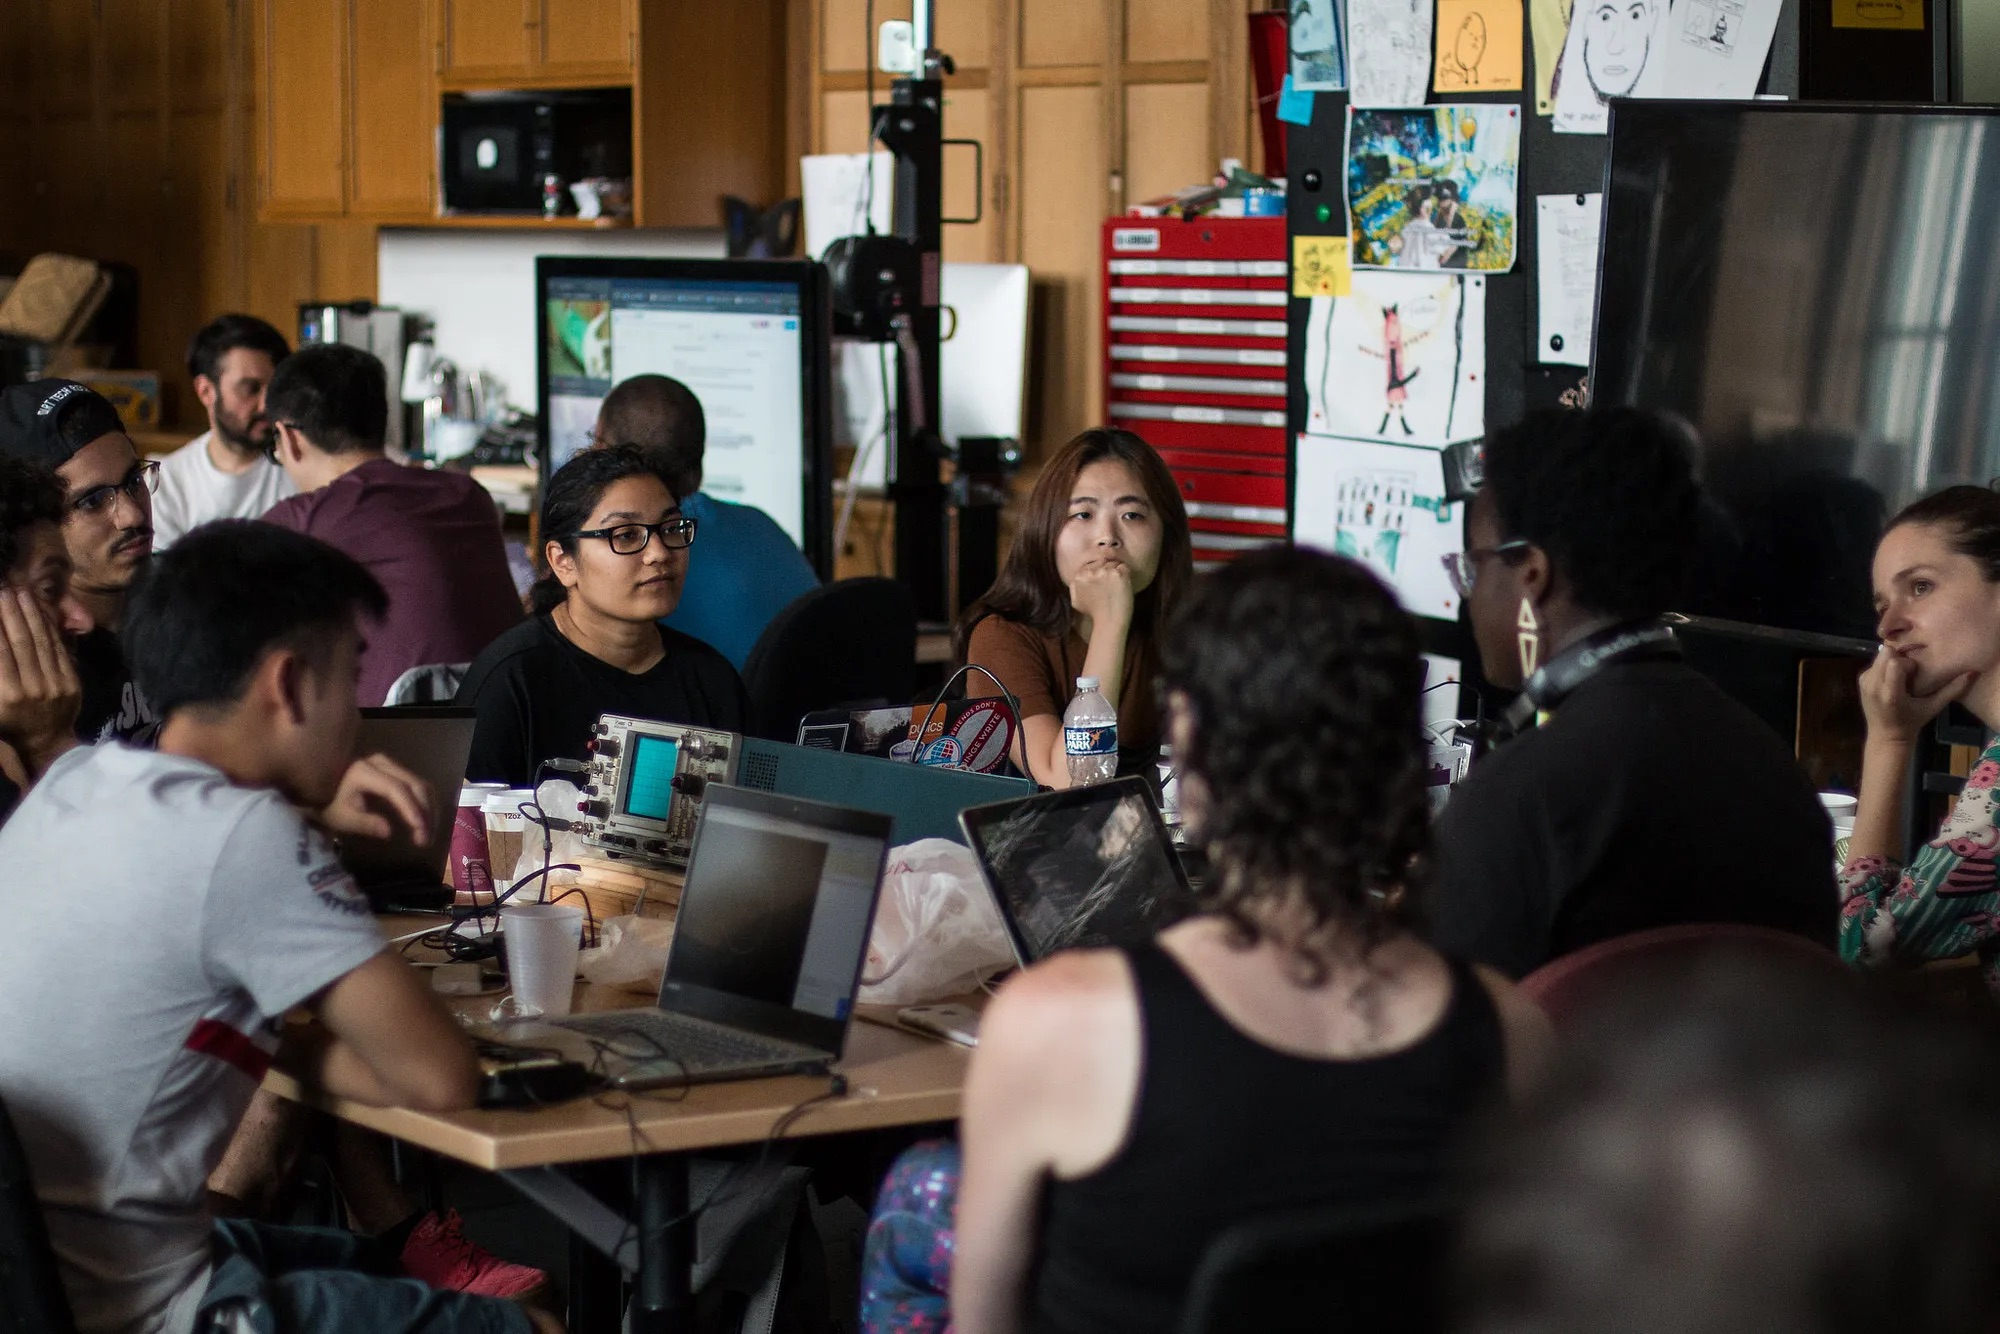
\includegraphics[width=\textwidth]{images/cathedral-or-bazaar.jpeg}
	\caption{Photograph from 2019 p5js Contributor Conference}
	\label{fig:p5ps-conference}
\end{figure}

\todo[inline]{Include image credit p5js project lead from zotero}

\subsection{Software Development Models}

In exploring the software development aspects of the Processing project, it is crucial to understand the underlying models and motivations that drive the contributions. This analysis begins by delving into two predominant models outlined in Eric S. Raymond's influential work "The Cathedral and the Bazaar" \parencite{CathedralBazaarMusings2002a}, followed by examining the taxonomy of motivations among open-source contributors.

Eric S. Raymond's "The Cathedral and the Bazaar" identifies two distinct methodologies in open-source software development. The Cathedral model, exemplified by early GNU projects under Richard Stallman, is characterized by meticulous planning and centralized control \parencite{StallmanGNUManifesto1985}. This model functions much like the construction of a cathedral, where a small group of experts crafts a complex, well-organized structure over a long period.

In contrast, the Bazaar model, which gained prominence with the development of the Linux Kernel, espouses a more decentralized approach. Spearheaded by Linus Torvalds, this model is akin to a bazaar, where contributors from diverse backgrounds bring in their unique contributions, leading to rapid iterations and an evolving software landscape \parencite{TorvaldsLinuxKernelDevelopment1991}. These two models represent endpoints on a continuum, with many real-world projects, including Processing, displaying characteristics of both.

While the Cathedral and Bazaar models provide a structural understanding of software development practices, exploring the reasons why individuals engage in these projects is equally crucial. The sustainability of open-source projects like Processing hinges on the continuous flow of software contributions. Without the active and sustained involvement of contributors, the long-term viability of such projects could be at risk.

To gain a deeper understanding of what drives these contributions, we turn to the established taxonomy by Bonaccorsi et al. \parencite{bonaccorsiComparingMotivationsIndividual2006} ~\ref{tab:taxonomy}. This framework categorizes the motivations behind open-source contributions into Economic, Social, and Technological domains. 

The following chapters analyse the dynamics and motivations of contributions to the core and libraries respectively. The analysis combines quantitative data from software releases and version control systems with insights from interviews with key code contributors.

\begin{table}
    \begin{tabularx}{\textwidth}{l l} 
    \toprule
    Motivation area & Micro level \\
    \midrule
    Economic & Monetary rewards \\
     & Low opportunity costs \\
     & Gaining a reputation among peers \\
     & Gaining future career benefits \\
    \midrule
    Social & Fun to program (Loving to code) \\
     & Altruism (gift economy) \\
     & Sense of belonging to the community \\
     & Fight against proprietary software \\
    \midrule
    Technological & Learning \\
     & Contributions and feedback from the community \\
     & Working with a bleeding-edge technology \\
     & Scratching a personal itch \\
    \bottomrule
    \end{tabularx} 
    \label{tab:taxonomy}
    \caption{Taxonomy of Individual Programmers’ Motivations. Adapted from \parencite{bonaccorsiComparingMotivationsIndividual2006}}
\end{table}

\subsection{Core Contributions}
% What are core contributors
The core contributions here refer to the code that was integrated into the main chunk of the program delivered to people, specifically not to libraries or adjancent things. This not including only the bagel model.

% Data and methods
The quantitative data here was the releases data, reconstructed from log files, and the version control history commit history . Limitations: the releaseses are sometimes grouped together and sometimes information is missing, especially in the beginning, as it was done manually. The version control system was also changed a few times, so the logs might not be consistent. 
The commit logs within the Processing project's GitHub repository, while rich with data, do not provide a complete visualization of early contributions. In an interview with Ben Fry, it was elucidated that contributions from various lab members, including those from Simon Greenwold, were indeed substantial in the project's formative years. These contributions, although crucial, are not conspicuously traceable through the GitHub interface. Fry explains that due to the constraints of the version control systems like CVS and Subversion used at the time, he personally committed code from other contributors, ensuring their efforts were acknowledged in the commit logs, even if not directly attributed in the repository's graphical interface.
It is important to note that the data over represents Ben's contributions in the beginning, mainly because of the limitations of proper crediting and integration due to the version control systems (CVS and later subversion being used at the time)
While things were in CVS, I had to do the commits myself, but always noted where things came from in the commit history. It improved a little with Subversion and Google Code, but only by a little. GitHub was the first meaningful change where it really helped with the collaborative side of development. 
It is worth noting that the logistics of releasing software were more complex in the early 2000s than they are today. As can be seen in Figure~\ref{fig:processing-cd} of a mini CD from October 2002 illustrates, distributing software was not as straightforward as pushing updates to a Git repository.

% Data to interviews
Interviews were conducted with Ben Fry, the software engineering lead, Karsten Schmidt (toxi), code contributor and active member, and Simon Greenwold, core contributor and also member of the Aesthetics and Computation Group at MIT at the time. These people were selected here because they can be seen among the few contributors during the activity time of the Alpha Forum as can be seen on figure XXX. \todo[inline]{Mention code contributions of toxi and Simon Greenwold}

\changepapersize{305.3mm:210mm}
\customtag{largepage}

{
	\LARGE
	\noindent Frequency of Releases\par
	\vspace{0.2cm}
}

\begin{multicols}{3}
	\noindent
	\begin{minipage}{\columnwidth + \columnsep}
		\begin{tabular}{|r|l|}
			\hline
			Descriptive statistics & Time between releases \\
			\hline
			count                  & 60                    \\
			mean                   & 20 days 15:11         \\
			std                    & 47 days 00:10         \\
			min                    & 0 days 00:00          \\
			25\%                   & 1 days 00:00          \\
			50\%                   & 3 days 00:00          \\
			75\%                   & 26 days 18:00         \\
			max                    & 338 days 00:00        \\
			\hline
		\end{tabular}
		\captionof{table}{Release statistics}
		\label{tab:release-statistics}
	\end{minipage}
	\columnbreak
	\noindent
	\begin{minipage}{\columnwidth}
		\frame{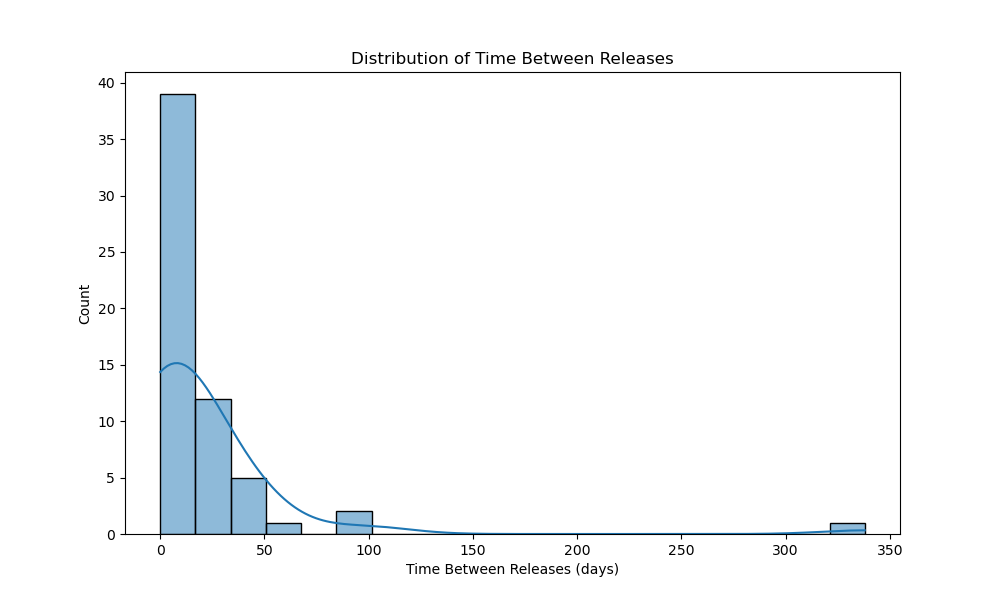
\includegraphics[width=\linewidth]{images/time_between_releases_histogram.png}}
		% \includegraphics[width=\linewidth]{graph2}
		\captionof{figure}{Graph that spans one column}
		\label{fig:releases-histogram}
	\end{minipage}
\end{multicols}

\begin{figure}[h!]
	\centering
	\frame{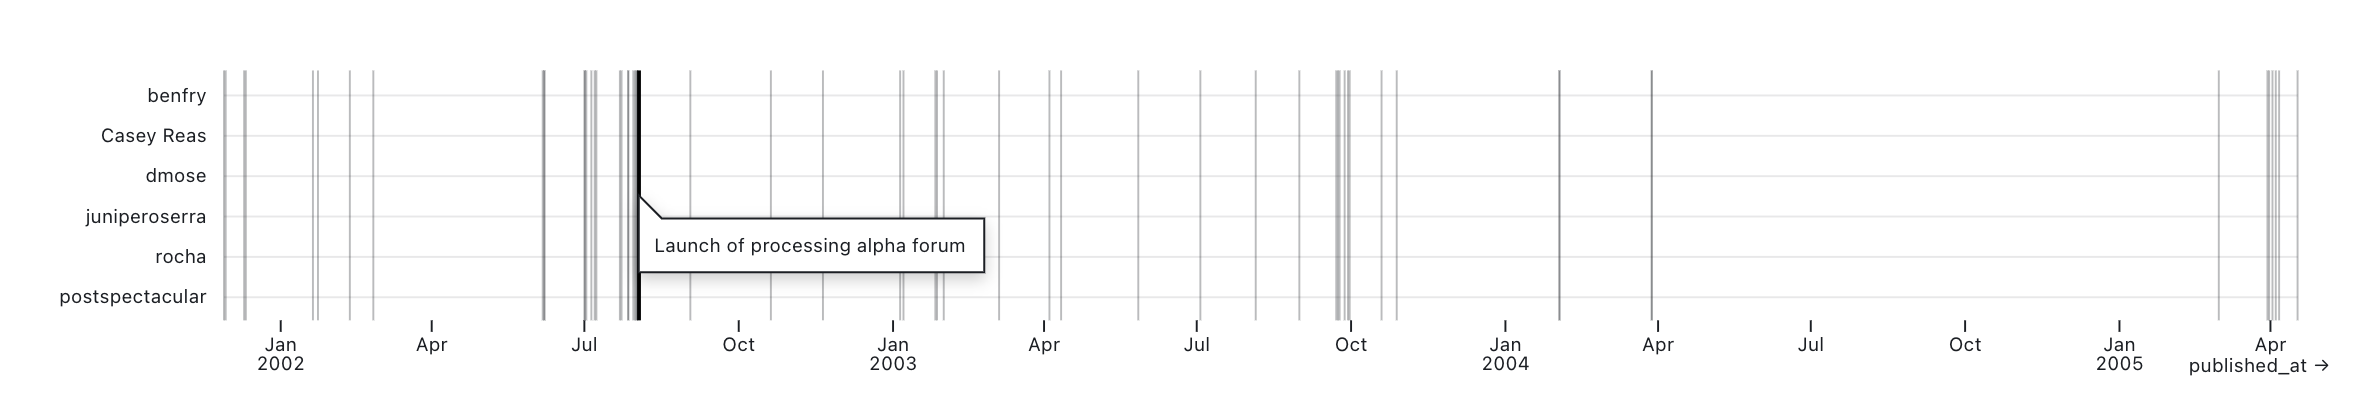
\includegraphics[width=1\textwidth]{images/releases-lines.png}}
	\caption{Time between releases}
	\label{fig:releases-lines}
\end{figure}

% \begin{figure}[h!] 
%   \centering
%   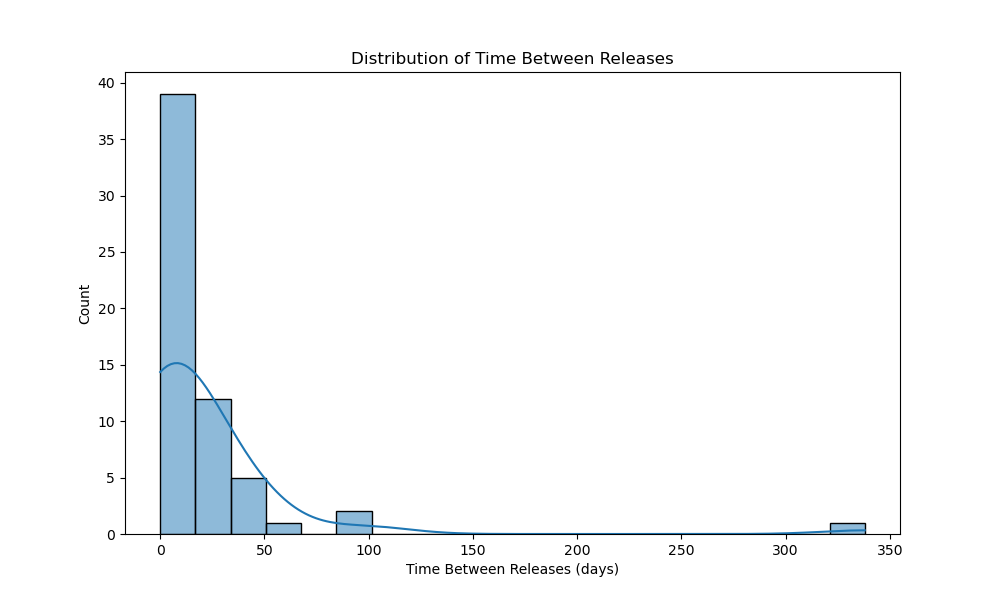
\includegraphics[width=0.9\textwidth]{images/time_between_releases_histogram.png} 
%   \caption{Time between releases histogram}
%   \label{fig:releases_frequency_histogram}
% \end{figure}

\begin{multicols}{3}
	\noindent
	The graphical representations depict a distinctive pattern of release clustering, a testament to the sporadic and intermittent nature of the project's development lifecycle. A notable surge can be observed leading up to pivotal milestones, such as the alpha forum's initial release, indicating a focused burst of activity during these critical junctures.
	\noindent
	The distribution of releases further accentuates the project's non-linear progress, with a marked increase in releases as key points approach, followed by periods of relative inactivity. This ebb and flow suggest that the development process is influenced by external factors or revolves around specific events, leading to a "feast or famine" scenario in terms of updates and improvements.
	\noindent
	Moreover, the extended intervals devoid of any releases could imply that the project advancement is perhaps a secondary or parallel endeavor for the contributors.
\end{multicols}

\defaultareasettings


\cleardoublepage
\changepapersize{305.3mm:210mm}
\customtag{largepage}

{
	\LARGE
	\noindent Version Control Statistics
}

\vfill

\noindent
	\begin{minipage}[t]{0.15\textwidth}
		\noindent
		\begin{figure}[H]
			\frame{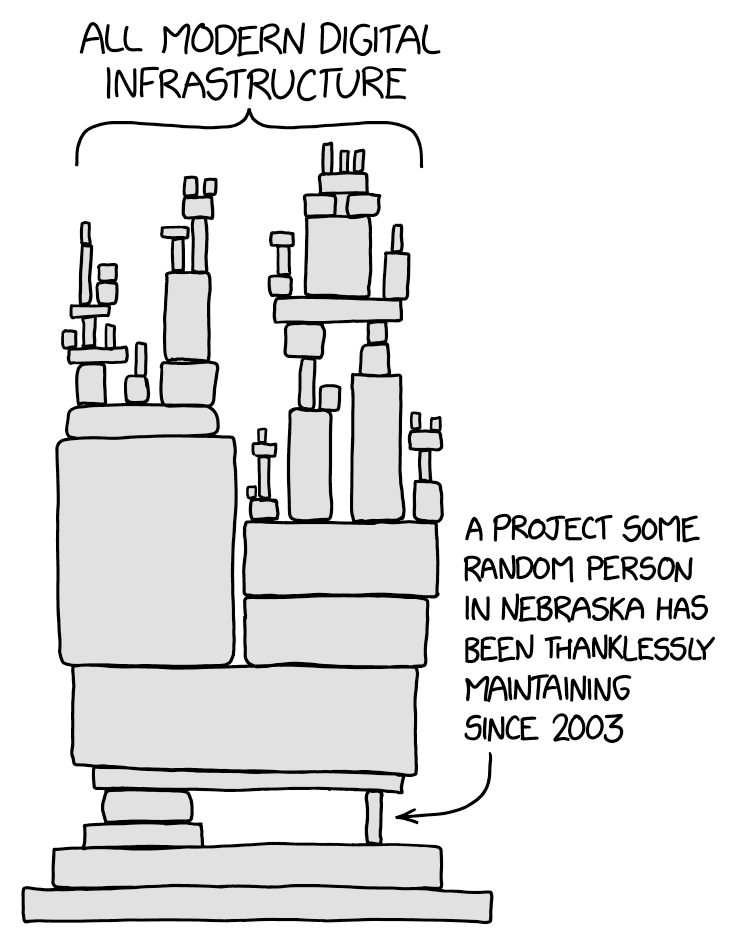
\includegraphics[width=\textwidth]{dependency.png}}
			\caption{Dependency comic}
			\label{fig:dependency_comic}
			% \small Source: \textit{XKCD}, \url{https://xkcd.com/2347/}, licensed under CC BY-NC 2.5.
		\end{figure}
	\end{minipage}
	\hspace{2mm}
	\begin{minipage}[t]{0.442\textwidth}
		\begin{figure}[H]
			\frame{\includesvg[pretex=\sffamily\fontsize{5.58pt}{8pt}\selectfont, width=\textwidth, keepaspectratio]{images/figure-top12-github.svg}}
			\caption[Top souce code contributors]{Top 12 source code contributors by number of commits in OCtober 2023}
			\label{fig:top12-github}
		\end{figure}
	\end{minipage}
\vspace{0.1cm}
\begin{figure}[H]
	\frame{\includesvg[pretex=\sffamily\fontsize{5.58pt}{8pt}\selectfont, width=1\textwidth, keepaspectratio]{images/processing-alpha-commits.svg}}
	\caption{Commits up to and including the Processing alpha forum}
	\label{fig:alpha-commits}
\end{figure}

\begin{multicols}{3}
	\noindent	
	The version control statistics portray a significant concentration of contributions by Ben Fry, indicating his pivotal role in maintaining the project across its timeline. The bar chart demonstrates Fry's preeminence through the sheer volume of his contributions relative to others. However, it's important to recognize that such visualizations do not fully encapsulate the breadth of contributions, especially in the project's nascent stages. Interviews suggest that many early contributions, made before the advent of sophisticated version control systems, remain unrepresented in these statistics. Thus, while the data underscores Fry's central involvement, it also omits a spectrum of foundational efforts that were integral to the project's initial development.
	\vfill\null
\end{multicols}

\defaultareasettings

% Initial Release: August 9 2001 -> Alpha Forum initial post: August 2 2002

In the development of the Processing project, Ben Fry's role as the main technical engineer was significant. This is underscored by the observations of his collaborators. Casey Reas emphasizes Fry's primary role: 'I think one thing that’s important to clarify is that Ben Fry, my collaborator, is the primary software engineer of the project' \parencite[p. 330]{conradGraphicDesignPostdigital2021}. Simon Greenwold further corroborates this, highlighting Fry's authoritative approach: 'He's maintaining strong control, like it's his code base. I think that's part of why it's great' (Greenwold, personal communication).

Completing the development of Bagel, the initial render engine, Ben Fry had established a robust code base a year before the debut of the processing alpha forum, prior to involving other contributors.

Fry discusses the early obstacles with MIT's Technology Licensing Office (TLO), particularly concerning intellectual property rights and the public release of the code. He details the extensive delays due to MIT, and more specifically the Media Lab, reevaluating their approach to open-source software, leading to an extended period of awaiting clearances.

Simon Greenwold underscores Processing's early adoption of an open-source model, a notable deviation in the context of Creativity Sustaining Toolkits (CST) for visual arts. He states, "Processing was notable in being open source early, ... probably unique in its class," thereby highlighting its pioneering role. In contrast, contemporaneous toolkits like Director or Flash were predominantly closed-source

Processing's development initially adhered to a centralized, cathedral-style model, characterized by structured, top-down control. The introduction of the alpha forum, however, marked a significant shift towards a decentralized, bazaar-style approach, encouraging community participation and collaborative code sharing.

This transition in Processing's development mirrors the early stages of other open-source projects like Linux, which also started with a solid foundation and evolved through community contributions. This shift to a more inclusive and collaborative model is a common trend in the development of open-source software.

The impact of this shift was evident in specific updates. The release notes from 27/05/2003 - rev 55, for instance, marked a turning point with the incorporation of code from external contributors, reflecting a move towards a community-driven development model. Following this, rev 56 further showcased the diversity of community involvement. It wasn't limited to code contributions; members engaged in various activities, including testing, providing feedback, and enhancing documentation. This broadened participation exemplified the multifaceted nature of the bazaar model, where contributions extend beyond programming to encompass various aspects of software development.

Note this as well "Treating your users as co-developers is your least-hassle route to rapid code improvement and effective debugging.” (Raymond, 1999, p. 27)

As the project evolved, Fry's role expanded to include the review and integration of contributions from other participants. He focused on preserving the simplicity of the project and making deliberate choices about what features to include, a strategy critical for the project's enduring success and practicality. \parencite{Processing4CONTRIBUTINGMd}

As more people wanted to develop different things for the project a library system was created. This is discussed more in detail in the following chapter. 

The maxim "Release early, release often," attributed to Eric S. Raymond in his seminal text "The Cathedral and the Bazaar" \parencite{raymondCathedralBazaar1999}, is often touted as a catalyst for vibrant open-source communities. In particular, projects like Linux have benefited from this approach, allowing rapid integration of contributions from a distributed network of contributors. This not only boosts the morale of individual contributors but also creates a dynamic and responsive development environment.

There were 162 revisions before the arrival of processing version 1 as can be seen on Figure~\ref{fig:releases-lines} and quantified in the Table~\ref{tab:release-statistics}. The beginning was characterised by more frequent releases, than later especially for version 4 where things were basically just maintenance mode. There were days with multiple releases “Release early, release often.” ([Raymond, 1999, p. 28](zotero://select/library/items/87U5FDLI)) ([pdf](zotero://open-pdf/library/items/UZP875I7?page=6&annotation=FTZT2TNQ))

“In those early times (around 1991) it was not u n k n o w n for him to release a new kernel more than once a day!” ([Raymond, 1999, p. 28](zotero://select/library/items/87U5FDLI)) ([pdf](zotero://open-pdf/library/items/UZP875I7?page=6&annotation=MZTGBGDD))

This wasn't helped by the side project nature of processing.  
Moreover, the project’s side-project nature is confirmed by revision comments such as one from 05/01/2003, which reads: "hopefully January 2003 will be a good month for p5, as I have a short bit of time to work on it [...] I hope to get a few revisions out this month so I can get back to my 'real' work." These comments illuminate that, for core contributors, Processing is not necessarily viewed as a full-time commitment.

The perception of Processing as a side project rather than a full-time commitment for its core contributors is corroborated through multiple channels. For example, a revision comment from May 1, 2003, highlights this sentiment, stating, ``hopefully January 2003 will be a good month for p5, as I have a short bit of time to work on it [...] I hope to get a few revisions out this month so I can get back to my `real' work.'' This observation is further substantiated by a 2021 study titled ``Graphic design in the post-digital age: a survey of practices fueled by creative coding,'' which notes that Processing began as a personal initiative and was largely developed during nights and weekends. The study further reveals that the project received indirect funding from MIT through Fry's graduate stipend, and from Interaction Design Institute Ivrea (IDII) through Reas's salary, again indicating its ancillary nature in the professional lives of its principal contributors~\parencite[396]{conradGraphicDesignPostdigital2021}.
The fact that it was part time meant that probably they didn't get as much engagemeng as could have been gotten.
“Linus was keeping his hacker/ users constantly stimulated and rewarded--stimulated by the prospect of having an ego-satisfying piece of the action, rewarded by the sight of constant (even daily) improvement in their work.”

---------------------
He noted that it was a really interesting project was all still very. young, there was a lot of stuff to do

The contribution landscape within the Processing project, as vividly illustrated in Figure~\ref{fig:alpha-commits}, further highlights Fry's central role. During the alpha forum phase, only six individuals actively contributed code to the repository, contrasting sharply with the over 1000 individuals engaged in forum discussions. As previously discussed, it is important to bear in mind the limitations of the version control system's depiction of contributions.

% Plan
% Describe and then analyse
% Analyse per segment or as a whole? 
% Get the lessons that are relevant from the cathedral and the bazaar
% Analyse by feature and add positives
% analyse contribution
% analysis according to the Cathedral / Bazaar model

% Source code imbalance

% Releases. Is this important? How does it compare? 
% Trends in git commits
The \textit{Processing} project illuminates a crucial challenge often faced by open source communities: the dependency on key contributors. In the case of Processing, Ben Fry's central role over the past two decades raises concerns about the project's resilience and sustainability. His substantial contributions create a high-risk situation termed the "bus factor" \parencite{BusFactor2023}, which indicates how vulnerable a project becomes when overly reliant on a single or a small number of contributors. This vulnerability is not unique to Processing, as such dependency models are commonly observed across open source projects, often humorously discussed in popular culture \parencite{munroeDependency2020}.
This discrepancy between the number of code contributors and forum participants is indeed profound, as corroborated by the subsequent visualizations ~\ref{fig:top12-github} and comic anecdotes ~\ref{fig:dependency_comic}. The limited number of contributors to the codebase and the concentrated responsibility on a few individuals amplify the bus factor risk, an issue that warrants deeper investigation and consideration for the long-term health of the project.

% Graphs - side project
% It was his code base
% Nature of development
% - Through teaching, workshops
% Part time basis, commits coming up on workshop dates
% Look at graph to show the development before the release of the forum
% Dynamics at the MIT Media Lab
% Analysis though the prism of the Cathedral model
% User motivations
% Read back Simon Greenwold interview
% Java tools for prototyping
% Technical background

From interviews, we can see that other contributors Simon Greenwold sometimes would have liked features to be developed in a different way, also Karsten Schmidt. \todo[inline]{Mention example} 

This dynamic is highly relevant of the Cathedral type of software development, through a carefully planned project lead implementing the main functionalities of the project, sometimes to the frustration of others. There were a lot of peopel that wanted functionalities outisde of the knowledge of the creators, lots of discussions so the libraries system was introduced, which will be discussed more in detail in later chapters.

% Motivations
for me personally is the motivation that comes from seeing really talented people

Personal itch
Although ironically, it wasn't really used at the Media Lab while we were there: John used it in a couple of the classes he taught, much to the griping of students who either wanted it to do more, or others who felt like they could build their own tools that were better. It wasn't until the years after I had left the Lab that it began to be used more commonly (i.e. in the later 2000s).

% 
The profiles of contributors were from people that already had vast experience with graphics and graphics programming. They might have sensed limitations to what processing was capable of and were thus more frustrated than beginner users who came into the fold later. Mention toxi: look what I could do with director

Motivations of these contributors:
Economic, Technological, Social
The main motivations for the creator Ben was an idea of a continuation of DBN, 

Tool for reseach ... 
As researchers, all those extra steps just got in the way: we already knew how to do those things, and it just made the process tedious. So with Processing, we wanted to get closer to just having things show up and work.

. There was this connection between what we wanted to teach (and what students wanted to learn) with DBN, that mirrored the things that were difficult or tedious when coding in C/C++ with ACU.
Responsability

Always intertwined with teaching purposes

I learned to code at a very young age because other people shared their code. This was before the open source movement, and concepts like “Free Software” were codified. It was just considered a normal and just way to do things at the time. So that was a major influence for me: paying forward what all those people had done for me. Their willingness to share, or even answer questions of a 9- or 10- or 12-year-old was a pretty incredible gift, and had a huge impact.

Examples from revision 56
net and video code was contributed by hernando barragan of ivrea
http://people.interaction-ivrea.it/h.barragan
everyone say "thanks hernando!"

the audio code is by carlos rocha, a hired gun whose 
employment was made possible by the generous support of ivrea. 
yay carlos! yay ivrea!

It is worth mentioning that the Processing project is different from the types of software analyzed in the Cathedral and the Bazaar. The software itself in this case is used to create other applications for designers and artists. In this sense processing can be categorised as a Creativity Sustaining Toolkit for visual arts. It is in essence a tool to create other things directly. The examples of the mail server analzed in the cathedral and the bazaar it is mereley an end user application that the user runs with a predictable end result.

A contributor in this sense to the project, would contribute code to evolve the software, but also in the mission of a low floow, high ceiling ethos encourage users to explore the limits of this system. Throgh the building of examples, contributing documentation, answering questions etc.

An interesting reference for this is more a communities of practice dynamic. 
Introduce communities of practice.
The fostering of the values spoken of in communities of practice can create a vibrant creative community that learns from itself, though it's interest, in what was primarily discussed as computational design at that time. They get better at it and create tools for other members of the community. Building and discussing in the open and commenting on each others work creates a dynamic that can be seen in an academic setting through peer review.

Open source software has evolved from a grassroots, community-driven activity into a mainstream phenomenon influencing all sectors of software development. This transition has been analyzed from numerous perspectives, including Etienne Wenger's theory of Communities of Practice, which posits that learning occurs in social contexts \parencite{wengerCommunitiesPracticeLearning1998}. This theory underscores the importance of shared experiences, tools, and discourse in shaping a community's collective practice. In the context of open-source software, these dynamics offer invaluable insights into the sustainability and progression of such projects. For instance, the Processing community exemplifies more than just a collection of individual contributors; it represents a dynamic community molded by common goals and collective learning.

However, through voices the Processing Foundation highlights that even though the bazaar model is percieved as an efficient way to develop efficient software, it is sometimes overvalued as an only way of making a contribution.

“Contributors recognize that writing code is not the only way to become a contributor; they think teaching, organizing community events, and creating tutorials and documentation are valuable ways of contributing and building community. One contributor that I talked to even suggested that perhaps final users should also be considered contributors because without them there would be no reason for developing or teaching p5.js.” \parencite[41]{processingfoundation20thAnniversaryProcessing2022}

This communal focus contrasts sharply with the software development models described in Eric S. Raymond's seminal work "The Cathedral and the Bazaar" \parencite{CathedralBazaarMusings2002a}. The Cathedral model is marked by careful planning and centralized authority, more akin to the early GNU projects initiated by Richard Stallman in the 1980s. Conversely, the Bazaar model encourages open collaboration and decentralization—features commonly associated with contemporary open source projects. These two models can be conceptualized as endpoints of a continuum, with real-world communities of practice, like the Processing community, potentially embodying characteristics of both.

Although Richard Stallman's Free Software Movement initially utilized a Cathedral-like approach, the evolution of version control systems like Git has facilitated the adoption of more decentralized, Bazaar-like models. This technological and philosophical shift intriguingly complements Wenger's notions of "mutual engagement," "joint enterprise," and "shared repertoire"—elements that nurture a sense of community and shared objectives \parencite{wengerCommunitiesPracticeLearning1998}.

To holistically grasp the intricate interplay of social and technical factors contributing to the success of open-source initiatives, a multidimensional analysis is essential. Such an approach would synthesize various frameworks, including Wenger's Communities of Practice \parencite{wengerCommunitiesPracticeLearning1998} and Raymond's Cathedral and Bazaar models \parencite{CathedralBazaarMusings2002a}, aiming to provide a nuanced understanding of a community's past, present dynamics, and future potential.

% in the following paragraph remove emphasis from the role of companies, mention that there is an interest in the motivations actors contributing to these projects because they mostly seem to lay in contrast with traditional economic normes - provide citation
% Economic Motivating Factors - While existing literature often focuses on the role of companies in contributing to open-source projects through complementary services like consulting, our study diverges by focusing on individual contributors. In the context of the Processing community, corporate involvement is notably lesser when compared to platforms like Linux that have substantial corporate contributions.

% The followind taxonomy is deemed interesting as a basis of analysis. Other frameworks exist, analysing the behaviour of comanies for example, but are not of interest for us
Building upon established frameworks such as the taxonomy by Bonaccorsi et al.~\cite{bonaccorsiComparingMotivationsIndividual2006}, which categorizes motivations behind open-source contributions into Economic, Social, and Technological domains, our study intends to adapt this taxonomy to suit the specific nuances of the Processing community.

\begin{figure}[h!]
	\centering
	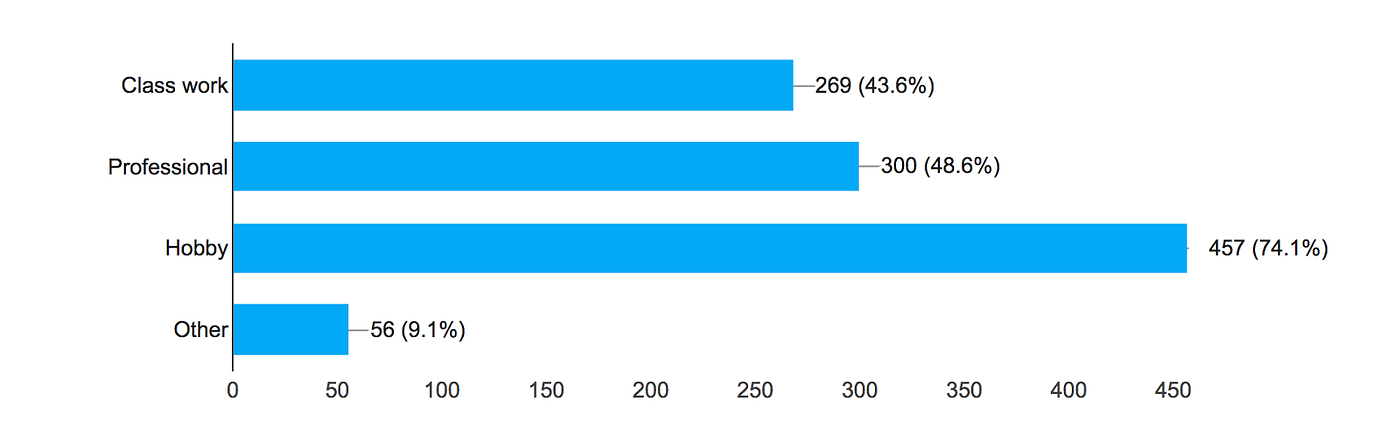
\includegraphics[width=\textwidth]{images/community-survey.png}
	\caption{Processing 2016 community survey result \parencite{2016CommunitySurvey}}
	\label{fig:community_survey}
\end{figure}
% Education
The 2016 Processing community survey revealed a significant number of users employ the language for educational purposes. This is consistent with Processing's design ethos, which is aimed at being educationally accessible. However, the extent to which this educational usage intersects with what can be termed as `professional use' remains unclear.

For the purpose of this study, `professional use' is understood to primarily include artists and designers. This nuanced categorization helps in probing the overlap between professional and educational use within the Processing community.

\subsection{An ecosytem of libraries}
\todo[inline]{Add Casey Reas quote}
An important milestone in the Processing ecosystem was the introduction of libraries. These libraries extended the functionalities of the base platform, thereby attracting a broader range of users and contributors. Such an analysis not only sheds light on the diversification of the project but also identifies key contributors and library authors who could potentially be sought out for qualitative interviews. The identification of these contributors adds another layer to our understanding of community participation.

Libraries have always been a crucial component of the Processing community, serving as essential building blocks that extend the platform's capabilities and foster creative exploration. Contributors to these libraries, like Ricard Marxer, Andreas Schlegel, and Karsten Schmidt, are not just developers; they are innovators who play a pivotal role in shaping the Processing ecosystem. Their motivations for contributing provide insightful perspectives into the diverse factors that inspire individuals to engage in open-source projects.

Ricard Marxer, the mind behind the 'geomerative' library, was driven by a blend of personal interest, community engagement, and the thrill of technological innovation. His enthusiasm for programming is evident in his creation of the geomerative library, which addressed specific needs in geometry processing within Processing. Marxer's comment, "I made generative for that, like it was the generative library for geometry," reflects his personal investment in solving technical challenges. Furthermore, his involvement in the community was not solely about personal achievement but also about being part of a larger group, as he fondly recalls the social aspects, "I really enjoyed going a lot to Madrid...and I get to meet all the people from the community of processing."

Andreas Schlegel, who created ControlP5, shows a different set of motivations. While not focusing on economic benefits, the social aspect of his work, particularly recognition within the community, was significant for him. Schlegel mentions, "I do get recognized for writing these libraries and for, by those who are familiar with the community and have used processing before." His contributions, initially experimental, reflected an altruistic intent to provide something useful to the community. Schlegel's journey from learning to contributing, "In the beginning, learning more through reading, and then after a while, I would then also help out and respond to questions that were coming in," highlights the importance of community interaction in driving motivation.

Karsten Schmidt's contributions to toxiclibs were deeply rooted in technological curiosity and a penchant for experimentation. His focus on software side projects and the technical aspects of programming are evident. Schmidt's involvement in early Processing development and creation of toxiclibs suggests a keen interest in working with new technologies. He demonstrated a broader interest in software development challenges, going beyond Processing to work with other languages and tools, as indicated in his discussions about various technical aspects.

The concept of "scratching a personal itch" emerges as a notable motivator for these contributors. They developed their libraries while addressing specific, personal needs or challenges, a common driver in many open-source projects. Marxer's development of the geomerative library, Schlegel's creation of ControlP5, and Schmidt's work on toxiclibs hint at this motivation, where the initial impetus to contribute often stemmed from their own experiences and requirements.

In summary, the motivations of library contributors in the Processing community are as diverse as their backgrounds. From Marxer's enjoyment of coding and community involvement to Schlegel's recognition within the community and Schmidt's technological curiosity, these motivations underscore the multifaceted nature of open-source contribution. Here, personal passions, community dynamics, and the thrill of technological innovation converge, highlighting the unique blend of personal, social, and technological factors that drive individuals to contribute to open-source projects like Processing.

\changepapersize{305.3mm:210mm}
\customtag{largepage}

{
	\LARGE
	\noindent Libraries releases
}

\begin{figure}[H]
	\includesvg[pretex=\sffamily\fontsize{5.58pt}{8pt}\selectfont, width=1\textwidth, keepaspectratio]{images/figure-libraries.svg}
	\caption{Distribution of Libraries in the Processing Project}
	\label{figure:libraries}
\end{figure}

\begin{multicols}{3}
	\todo[inline]{Shorten this explanation, or move some parts elsewhere}
	\noindent
	This graph illustrates the distribution of Processing library releases over a period from January 2012 to April 2014. Each dot on the graph signifies a release event for a library in various categories such as 3D, Animation, and GUI. The process of releasing these libraries was manual, requiring approval on the Processing website before they became available for update. This artisanal method meant that only the latest versions of the libraries were accessible, without an option to retrieve previous iterations.
	\noindent
	The data for this graph was meticulously reconstructed using a 'git blame' operation on the data folder containing links to these libraries. It's worth noting that this data may not fully represent the entirety of the Processing library space. The reconstruction is based on a single version of the website's data, lacking a comprehensive historical record that could have been obtained from multiple website versions. Thus, while the graph provides valuable insights into the release patterns and activity within the Processing community, it comes with the caveat of being an incomplete representation due to the availability of only one snapshot of the website data.
	\noindent
	In the context of the Processing community, this graph serves as a historical lens, capturing the cadence of library updates and highlighting the active categories of development. Despite the limitations in data scope, it reflects a significant portion of the community's contributions and the evolution of library offerings during the specified timeframe.
\end{multicols}
\defaultareasettings
